The synthetic nervous system controller is developed with a <insert name here>
neuron model. The neurons are modeled with a resting potential of -60 mV and a
maximum potential of -40 mV for a range of 20 mV.

% TODO(buckbaskin): make the capitalization of the networks consistent

\bbs{Key Neurons and Synapses}

The neuron controller network is made up of a set of engineered synapses
designed to emulate arthimetic operations. These can be grouped into two
categories: excitatory neurons and inhibitory neurons. Most neurons were tuned
via an optimization process to identify the best equilibrium potential and
synaptic conductance. Some neurons were tuned by hand for specific behaviors in
a subsection of the overall controller.

\bbss{Excitatory Synapses}

Except where otherwise noted, a value of 134 mV was used for the equilibrium
potential. The pre-synaptic threshold is -60 mV and the pre-synaptic saturation
level is -40 mV.

\bbsss{Signal Transfer}

The signal transfer synapse is designed to pass the voltage of the input neuron
to the output neuron in the active range of the neuron. It is often used to add
the value of two or more neurons together in an output neuron.
It has a synaptic 
conductance of 0.115 microsiemens. 

\bbsss{Inverted Signal Transfer}

By combining two signal inversions, a more accurate signal transfer synapse was
created. This involves an extra neuron; however, it leads to a more precise
transfer of the voltage level of the input neuron to the output neuron. In
general, the synapse was implemented with two Signal Inverter (Stimulated)
synapses.

\bbsss{Signal Amplifier 2x}

The signal amplifier synapse is designed to pass the voltage of the input neuron
to the output neuron with a 2x gain. This was tuned with input values from 0 to
10 mV. Higher inputs saturate the output neuron. It has a synaptic conductance
of 0.23 microsiemens.

\bbsss{Signal Amplifier 4x}

The signal amplifier has the same function as the 2x amplifier but with a x4 
gain. This was tuned with input values from 0 to
5 mV. Higher inputs saturate the output neuron. It has a synaptic conductance
of 0.46 microsiemens.

\bbsss{Signal Reduction 0.2x}

The signal reduction synapse is designed to pass the voltage of the input neuron
to the output neuron in the active range of the neuron, but with a loss of 0.2x. 
It has a synaptic  conductance of 0.021 microsiemens. This neuron was tuned
over the complete range of input values, 0 to 20 mV.

\bbsss{Signal Reduction 0.5x}

The signal reduction synapse is designed to pass the voltage of the input neuron
to the output neuron in the active range of the neuron, but with a loss of 0.5x. 
It has a synaptic  conductance of 0.054 microsiemens. This neuron was tuned
over the complete range of input values, 0 to 20 mV.

\bbsss{Convert Forward Positive}

The convert forward positive synapse is designed to convert the representation
of a value in a single neuron, for example the neuron that represents the 
position of the joint, to the same value represented in two neurons. This
synapse converts the value when the value is above -50 mV to values between 0 
and 20 mV. The pre-synaptic
threshold is -50 mV and the synaptic conductance is 0.115 microsiemens.

\bbsss{Torque Pressure Converter}

The torque pressure converter synapse is designed to perform the torque-pressure
calculation approximation. It has a synaptic 
conductance of 0.048 microsiemens.

\bbss{Inhibitory Synapses}

Except where otherwise noted, the equilibrium potential of inhibitory neurons
is simulated as -100 mV. This is the lowest value possible in the simulation.
The pre-synaptic threshold is -60 mV. The pre-synaptic saturation level is -40
mV.

\bbsss{Signal Inverter}

The signal inverted synapse is designed to decrease the voltage of the output 
neuron proportional to the voltage of the input neuron. It has a synaptic 
conductance of 0.55 microsiemens.

\bbsss{Signal Inverter (Stimulated)}

The signal inverted synapse is designed to decrease the voltage of the output 
neuron proportional to the voltage of the input neuron. This synapse is tuned
slightly differently from the standard signal inverter because there was an
observed difference in voltage when a stimulus current was applied to the output
neuron along with other incoming synapses. It has a synaptic 
conductance of 0.5 microsiemens.

\bbsss{Signal Invert Reduction 0.2x}

The signal inverted reduction synapse is designed to decrease the voltage of
the output 
neuron at a 0.2x loss compared to the voltage of the input neuron. It has a 
synaptic conductance of 0.093 microsiemens.

\bbsss{Signal Invert Reduction 0.5x}

The signal inverted reduction synapse is designed to decrease the voltage of
the output 
neuron at a 0.5x loss compared to the voltage of the input neuron. It has a 
synaptic conductance of 0.22 microsiemens.

\bbsss{Signal Inverter Amplifier 2x}

The signal inverted amplifier synapse is designed to decrease the voltage of
the output 
neuron at a 2x gain to the voltage of the input neuron. It has a synaptic 
conductance of 1.11 microsiemens.

\bbsss{Signal Inverter Amplifier 4x}

The signal inverted amplifier synapse is designed to decrease the voltage of
the output 
neuron at a 4x gain to the voltage of the input neuron. It has a synaptic 
conductance of 2.3 microsiemens.

\bbsss{Integral Inhibitor}

The integral inhibitor synapse is designed to help both neurons maintain a 
stable value unless an external current is applied. The values for this
synapse are based on \cite{NickFunctionalSubnetwork}. The synapse has a  
conductance of 0.5 microsiemens.

\bbsss{Convert Forward Negative}

The convert forward negative synapse is designed to convert the representation
of a value in a single neuron, for example the neuron that represents the 
position of the joint, to the same value represented in two neurons. This
synapse converts the value when the value is below -50 mV to a positve value 
from 0 to 20 mV. The pre-synaptic
saturation is -50 mV and the synaptic conductance is 0.5 microsiemens.

\bbsss{Signal Divider}

The signal divider synapse is designed to reduce the effect of another input
synapse, where the reduction increases with increased input voltage to the
signal divider synapse. It is distinguished from the signal multiplier synapse
in that the value never reaches 0. Intuitively, this is a replication of 
division where dividing by a large number makes the quantity small but never 0.
It has a synaptic conductance of 20 microsiemens. The equilibrium potential of
the synapse is -60 mV (equal to the resting potential of the input and output
neurons).

\bbsss{Signal Multiplier}

The signal divider synapse is designed to reduce the effect of another input
synapse, where the reduction deccreases with increased input voltage to the
signal divider synapse. It is distinguished from the signal divider synapse
behavior in that the value reaches 0. Intuitively, this is a replication of 
multiplication where multiplying by 0 will make any value 0.
It has a synaptic conductance of 19.75 microsiemens. The equilibrium potential 
of the synapse is -61 mV.

\bbs{Sensor Fusion}

The Sensor Fusion neuron network performs essentially the same function as the
sensor fusion network in the prototype controller. In this case, 3 neurons
represent the 3 sensor inputs available in a joint: position (``Theta"),
extension muscle pressure (``Ext Pres") and flexion muscle pressure
(``Flx Pres"). The outputs for the network are the estimates for current 
position, velocity and acceleration.

\bbss{Velocity Fusion Network Components}

\bbsss{Differentiator Network}

% 2
% TODO(buckbaskin): talk about differentiator network
The velocity network is based on the Differentiator Network presented in 
\cite{NickFunctionalSubnetwork}.

% 3
% TODO(buckbaskin): Figure of differentiator network

\bbss{Velocity Fusion Network}

The velocity network is based on the Differentiator network. 
The one major change from the network,
as presented, is the inclusion of a second $U_{post}$ neuron to represent the
negative derivative of the position (negative velocity).

% 4
% TODO(buckbaskin): Figure of my velocity network

% TODO(buckbaskin): make sure my inhibitory and excitatory synapses are visualized properly

This represents
a common pattern used across the network where two neurons are used to represent
a single value. One neuron represents positive levels of the variable and is 
at or below resting potential when the value is negative. The other neuron is
above resting potential for negative values and is at or below resting potential
when the value is positive. 

The motivation for increasing the complexity of the
network (often making it more than twice as complicated) is to increase the
effective range of values that the neuron can represent at the same fidelity and
to increase the accuracy of zero. When a single neuron represents positive and
negative values of equal magnitude, the value of 0 is represented at 50 mV; 
however, after passing through a signal transfer synapse this value is often
slightly higher, up to 52 mV. This means that comparing the two neurons (the
original neuron and the signal transfer) yields a slightly positive error
instead of near zero error.

\bbss{Acceleration Fusion Network Components}

\bbsss{Absolute Value Network}

Within the acceleration fusion network, the absolute value of the position is
used. This is calculated by first splitting the position into its two neuron
representation. From there, the sum of the two neurons is used as the absolute
value. This takes advantage of the definition of each side of the two neuron
representation falling below resting potential when the other neuron is active.
This means the signal transfer synapse from the below zero neuron will have no
effect.

% 5
% TODO(buckbaskin): Figure of my absolute value network

\bbsss{Integration Network}

The integration network used throughout the neuron controller is based heavily
on the Integrator Network in \cite{NickFunctionalSubnetwork}. Two neurons are
designed to mutually inhibit each other so that the combined pair hold their
values. Individual neurons can be treated as a leaky integrator; however, their
voltage tails off over time if there is no maintenance current. The integration
network itself is tuned by changing the time constant of the component neurons
to adjust how much the voltage of the integrator network changes for an input
current.

\bbsss{Convert Torque to Pressure}

% 6
% TODO(buckbaskin): talk about how this approximation came about through simulation
Linearized approximation to help with neurons

% TODO(buckbaskin): regenerate the PressureTorque figure with axis labels
\begin{figure}[h!]
\centering
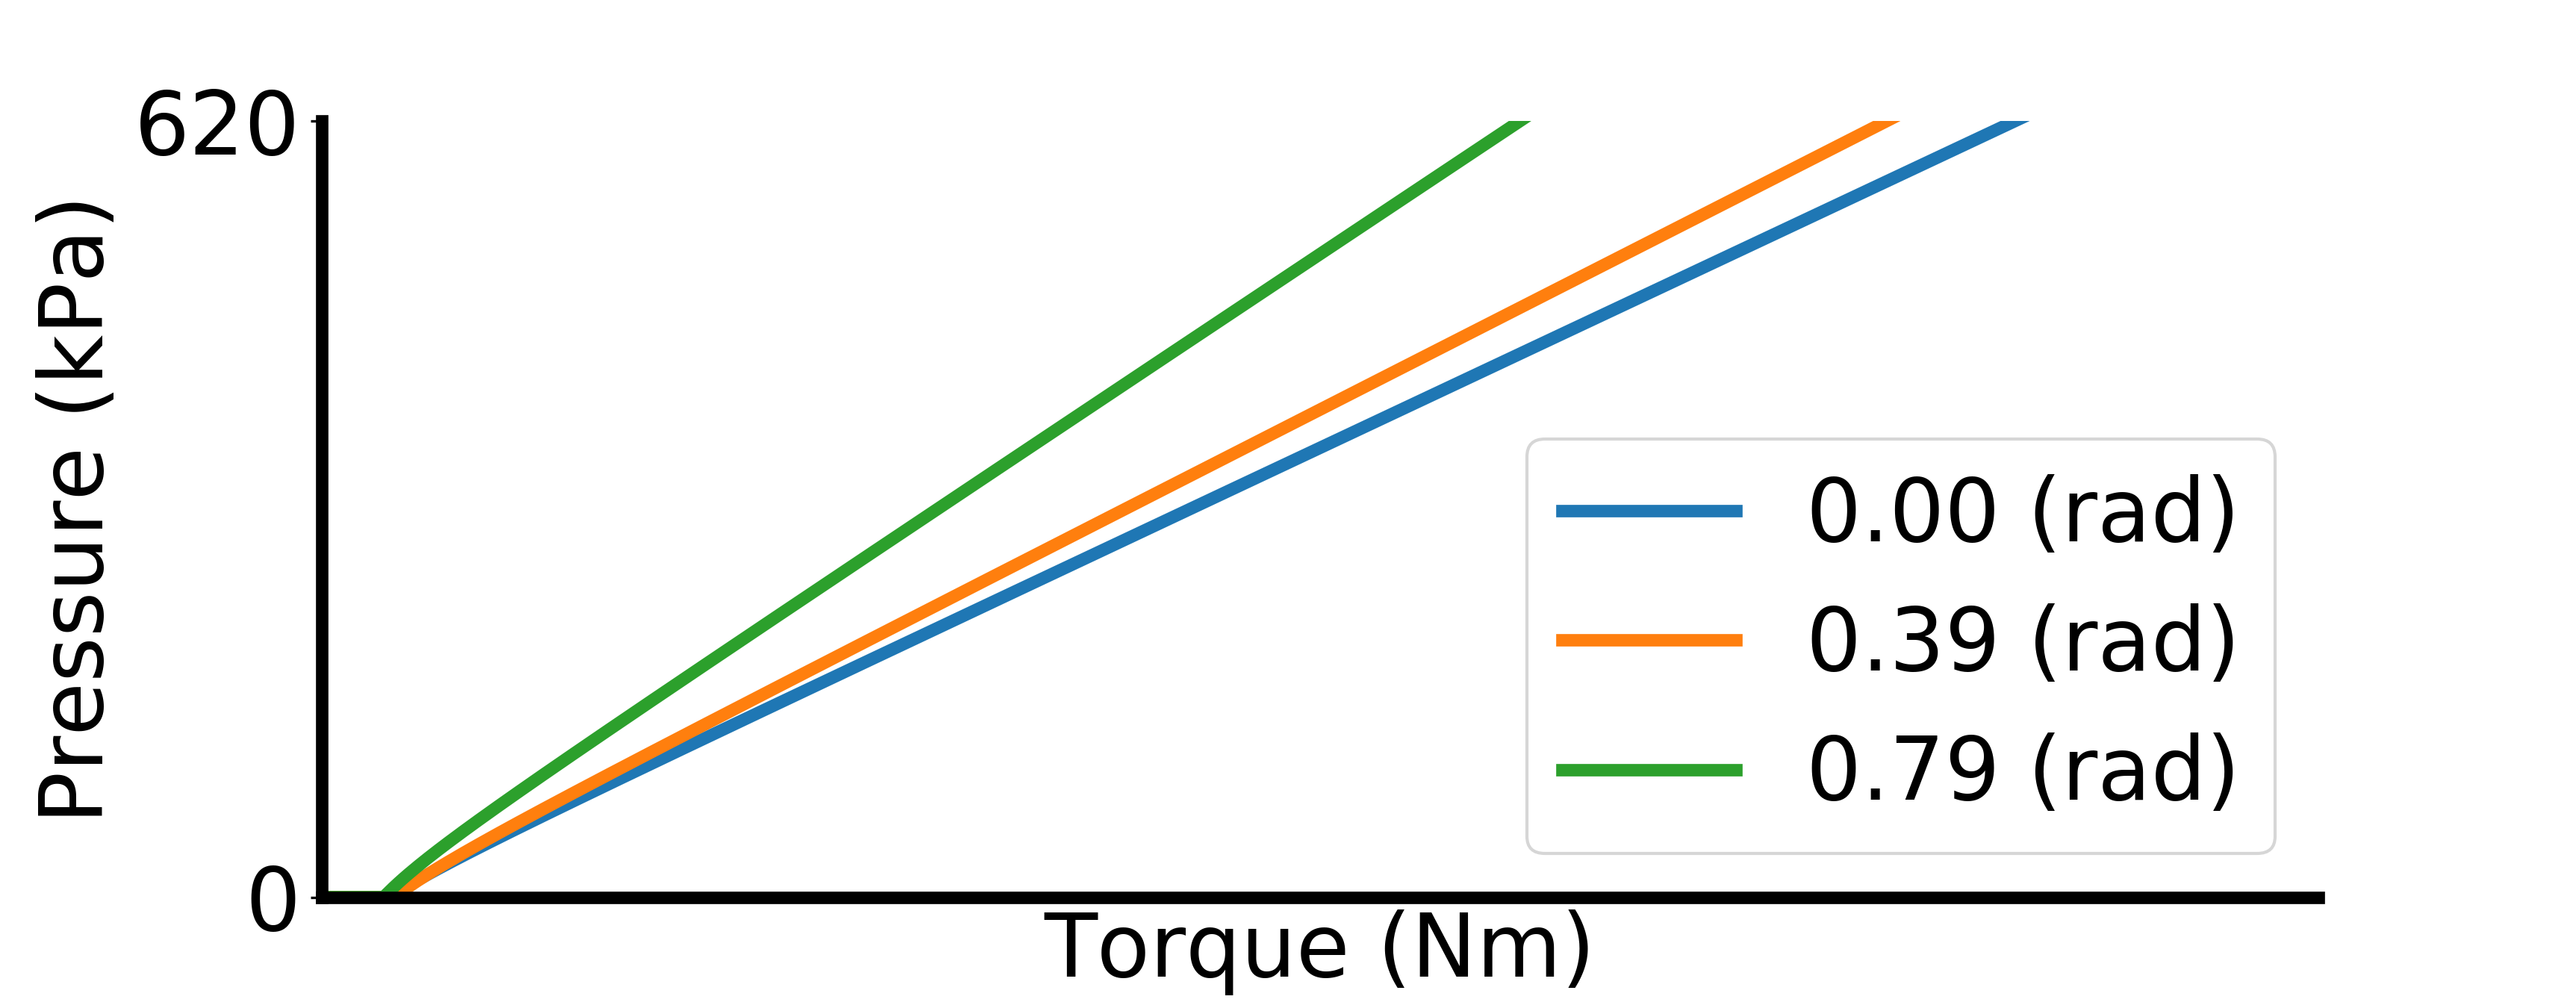
\includegraphics[width=5in]{neuron_design/FigPressureTorque}
\caption{Torque/Pressure relation observed in simulation}
\label{fig:PressureTorque}
\end{figure}

\bbsss{Pressure Estimation Loop}

Within the Acceleration Network, there is a feedback loop that is used to 
estimate the torque applied by a given pressure. First, the loop ``initializes"
with an extension torque guess from the integrator. Second, the extension
torque is converted into extension pressure. Third, the estimated extension
pressure is compared with the sensed pressure. If there is an delta between the
two, the extension torque guess is modified in turn and the cycle repeats.

% 7
% TODO(buckbaskin): Figure of pressure loops

This architecture is mirrored for flexion torque.

\bbss{Torque to Acceleration Network}

% 8
% TODO(buckbaskin): talk about T2A

\bbss{Acceleration Fusion Network}

The acceleration fusion network is a combination of an integrator, absolute
value network, the pressure estimation loop and a torque to acceleration
network. In total, the network uses a combination of smaller networks to
estimate the torque applied from sensed pressure and then combine the extension
and flexion torques together to get a net torque and acceleration.

\section{Optimizing Torque Control}

% 9
I/O summarizing, goals
position, velocity, desired position -> torque

\subsection{Small Networks}

% 10

\subsection{Mid Networks}

% 11

\subsection{Entire Network}

% 12

\section{Torque to Pressure}

% 13
I/O summarizing, goals
convert desired torque pressure in neurons

\subsection{Small Networks}

% 14

\subsection{Mid Networks}

% 15

\subsection{Entire Network}

% 16

\section{System Modeling}

% 17
I/O summarizing, goals
Parameter weight updates

\subsection{Small Networks}

% 18

\subsection{Mid Networks}

% 19

\subsection{Entire Network}

% 20

\bbs{Combined Controller Network}

\begin{figure}[h!]
\centering
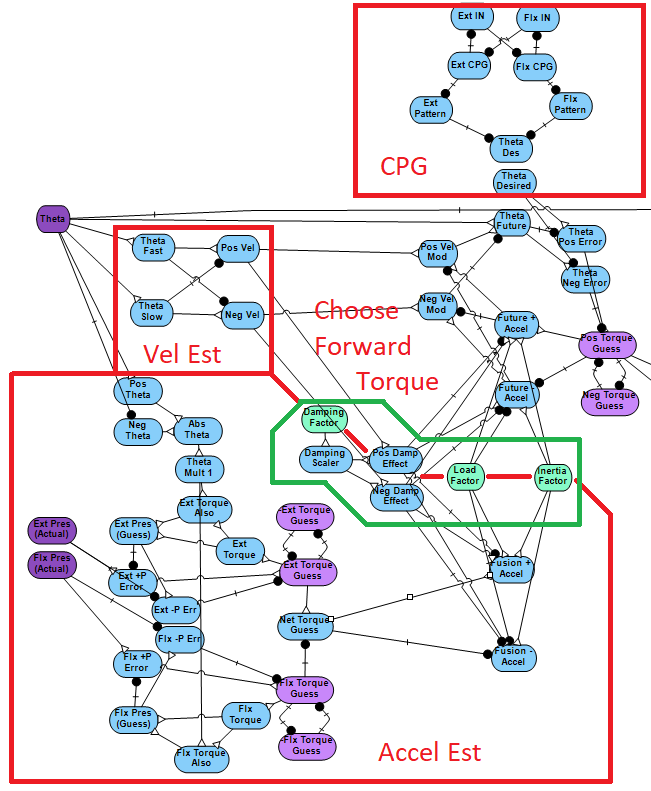
\includegraphics[width=5in]{neuron_design/NetworkLayout}
\caption{Overview of major network components}
\label{fig:NetworkLayout}
\end{figure}
% TODO(buckbaskin): redo this with the complete actual network